\section{Database}
%\subsection{stuff}

%\subsection{database}

	\begin{frame}{What? - Metadata of a task}
		\begin{itemize}
		\item Identifier(ID)
		\item Timestamp of an event
		\item Event itself
		\item Mode
		\item Parent
		\item Rank
		%\item Intercommunication timestamp
		\item Number of parameters
		\item Parameters themselves
		\end{itemize}
	\end{frame}
	
	\begin{frame}{How? - Structure}
		\begin{itemize}
		\item Stored data in 2 seperated files
		\item Bookkeeping: listed data of previous slide
		\item Statistics: parameters and runtime of a task
		\item Files are accessable for visualizer
		\end{itemize}
	\end{frame}
%\subsubsection{handling}
	\begin{frame}{DatabaseHandler}
	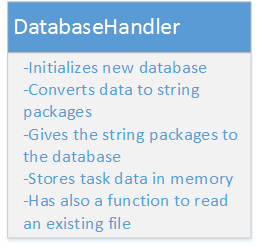
\includegraphics[width=0.3\textwidth]{images/databasehandler.png}
	\begin{itemize}
		\item Provides methods for data parsing
		\item Passes data through
		
	\end{itemize}
	\end{frame}
	
	\begin{frame}{DatabaseServer}
	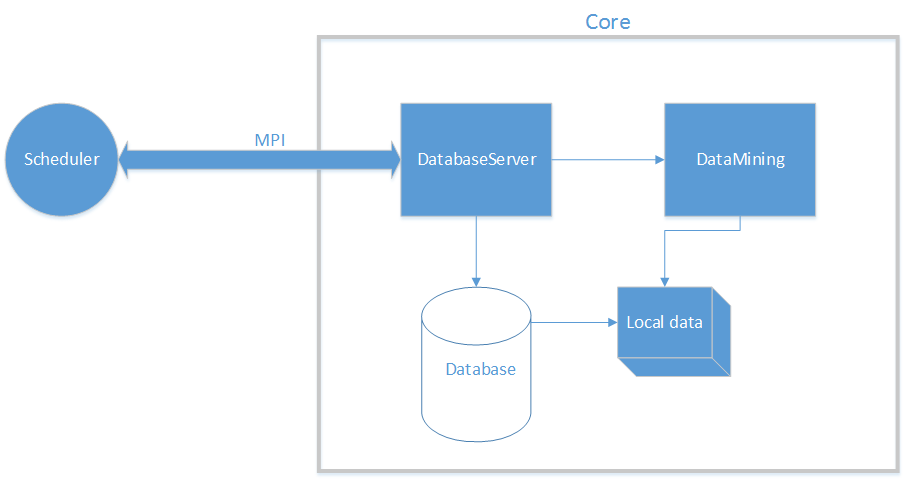
\includegraphics[width=1.0\textwidth]{images/Zeichnung6.png}
	\end{frame}
	
	\begin{frame}{Database - DataMining}
	\centering
	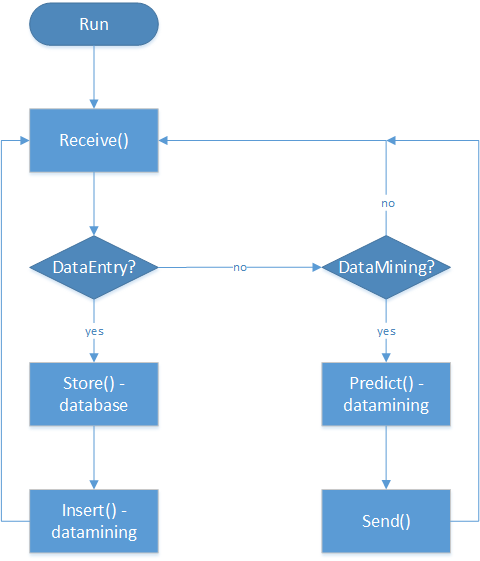
\includegraphics[width=0.55\textwidth]{images/datamining_flow.png}
	\end{frame}
